\let\textcircled=\pgftextcircled
\chapter{Introducing the Kalman Filter}
\label{chap:introkalmanfilter}

\initial{W}hen looking at combining data from various sources to provide estimates better than could have been achieved from each piece of data individually, there are currently four main algorithms to choose from; the central limit theorem, Bayesian networks, Dempster-Shafer theory or the Kalman filter.\par

%=======

\section{Filter Options}
\label{sec:choosingafilter}
	The central limit theorem is derived from probability theory and posits that for a large number of independent uniformly distributed events with well defined mean and finite variance, their mean will tend towards a normal distribution \cite{rice2006mathematical}. This theory is not applicable to the project as the number of data points per iteration will be fairly small, and both the mean and variance will change as the drone moves.\par
    Bayesian networks, otherwise known as Bayes networks or belief networks, are probabilistic directed acyclic graphs \cite{charniak1991bayesian}. Although most often seen using binary true/false examples, Bayesian networks can be equally used for variables with either discreet or non-discreet values. One of the main uses for Bayesian networks is to predict the unknown values of nodes in the network using known nodes that the unknown node is dependent on such as the example shown in figure \ref{fig:BayesianNetwork}. In this project however each measurement will be assumed to be independent and so the effectiveness of a Bayesian network would be very minimal.\par
\begin{figure}[t!]
	\centering
	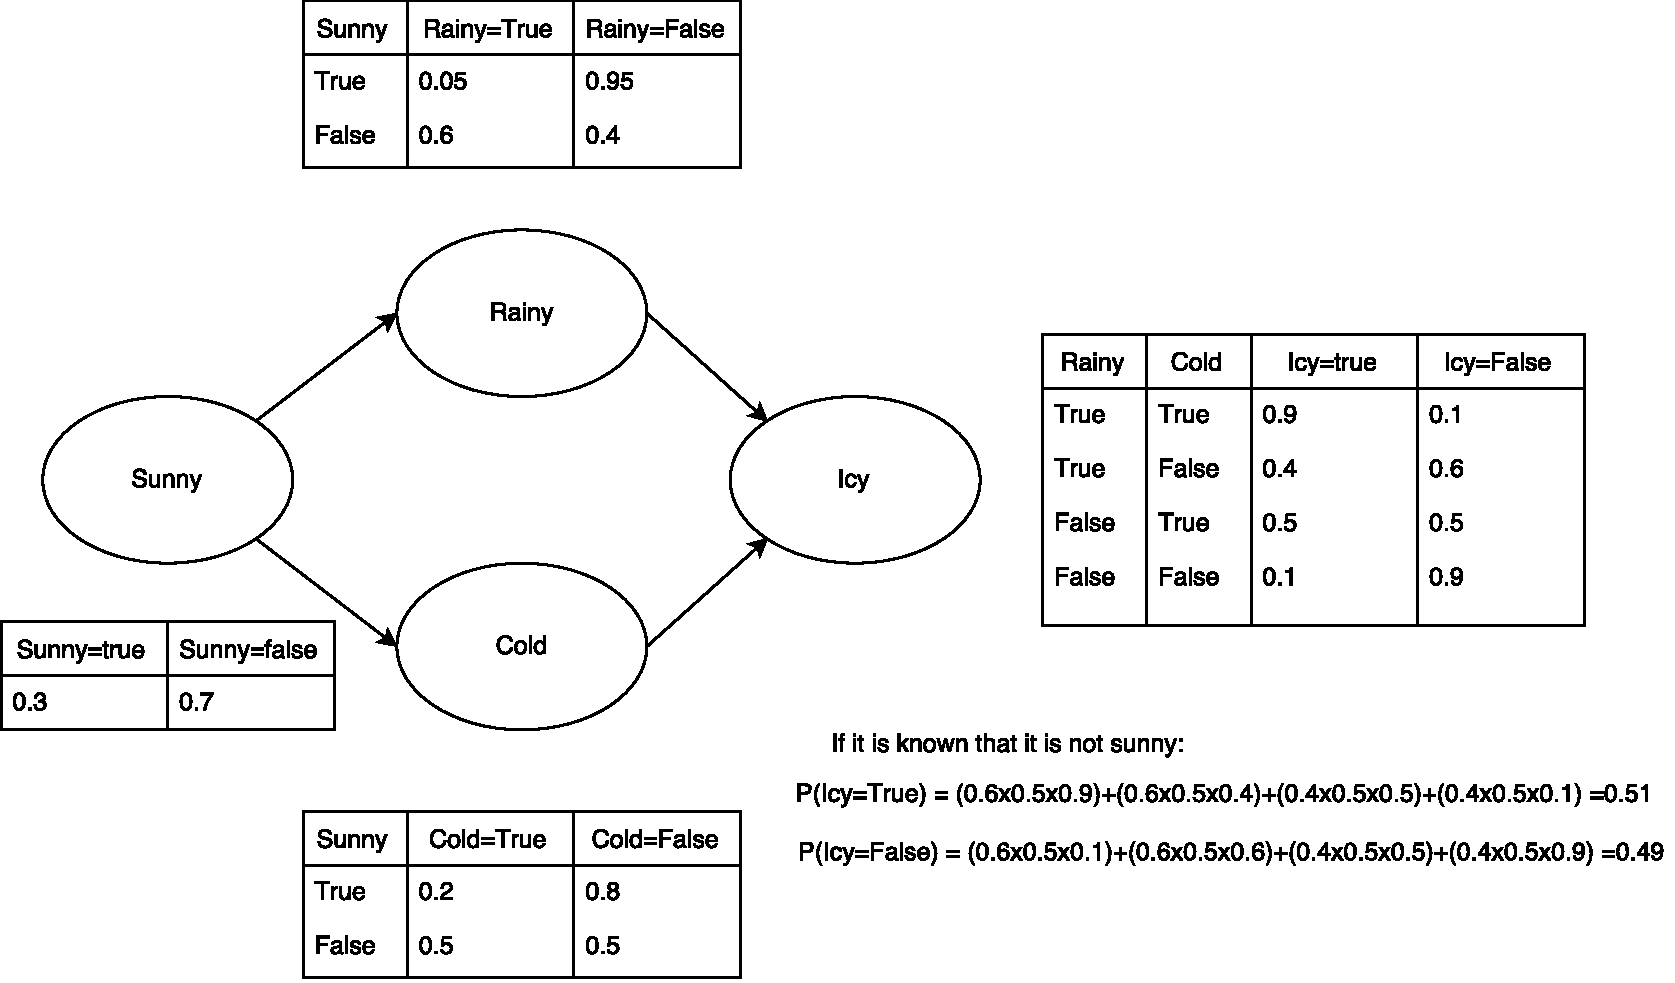
\includegraphics[height=0.45\textheight]{BayesianNetwork.pdf}
	\mycaption[Bayesian Network Example]{Diagram and calculations for a simple Bayesian network.}
	\label{fig:BayesianNetwork}
\end{figure}
	The Dempster-Shafer theory considers itself a generalisation of the Bayesian network algorithm where independent questions (nodes) also have a plausibility based on the probability of a related question. This "plausibility" is fundamentally different to a probability distribution characterised by belief, describing not the likelihood of a statement being true but instead describing to what degree similar question's results would influence the initial question's certainty \cite{shafer2002dempster}. This theory could yield a suitable sensor fusion implementation however it is overly complex for this situation. DST is designed to deal with a degree of ignorance caused by incomplete data or sensors that are not well modelled, a scenario that should be mitigated in this situation through proper sensor characterisation. \par
    The Kalman filter takes independent measurements of values, along with their known variance, and combines them to provide a new estimate with a lower variance \cite{kalman1960new}. This algorithm most closely matches the problem scenario and will be the one utilised going forward. Several non-linear variants of the Kalman filter exist which do not require state transition or observation models that are linear functions of the state. They are however substantially more complex, generally don't return an optimal estimate and are susceptible to divergence \cite{lefebvre2004kalman}. For the short-range sensors used, their response can generally be assumed to be linear. The GPS and IMU units do have linear error so will also not require a non-linear filter.
    
\section{Explaining the Kalman Filter}
\label{sec:kalmanfilterbasics}
Developed by Rudolf E. K\'{a}lm\'{a}n and published in 1960, the filter uses Bayesian inference and joint probability distribution to estimate new data in discreet time. The algorithm uses two principal steps; prediction of the new state from the old state along with any system inputs, followed by incorporation of all measurements taken. At all times the variance, or uncertainty, of the system is stored. Although this variance is not assumed to necessarily be Gaussian, it does yield an exact conditional probability estimate for that case \cite{kalman1960new}. \par
	In essence the process can be thought of as a form of weighted averaging where extrapolations or measurements with more certainty are given higher weighting. 

	The Kalman filter sees the world as a collection of variables with Gaussian distributed values and relies upon combination of these distributions to function; figure \ref{fig:gaussiancombination} shows graphically how two probability distributions are multiplied together to obtain a tighter distribution. Therefore key to understanding and implementing the filter is proper characterisation of the state and measurements. The state is the filter's representation of the variables to be estimated with a mean \(\mu\) representing the best estimate. Each state item also has a variance \(\sigma^2\) modelling the uncertainty in the measurement. Since the variance for one data item might influence the estimated value of another, the variances are combined into a symmetric covariance matrix which accounts for this \cite{babb2015how}\cite{faragher2012basis}\cite{simon2001kalman}. For instance the estimated distance is correlated to the measured velocity and vice versa, this allows additional information to be retrieved from each sensor reading.\par

\begin{figure}[t!]
	\centering
	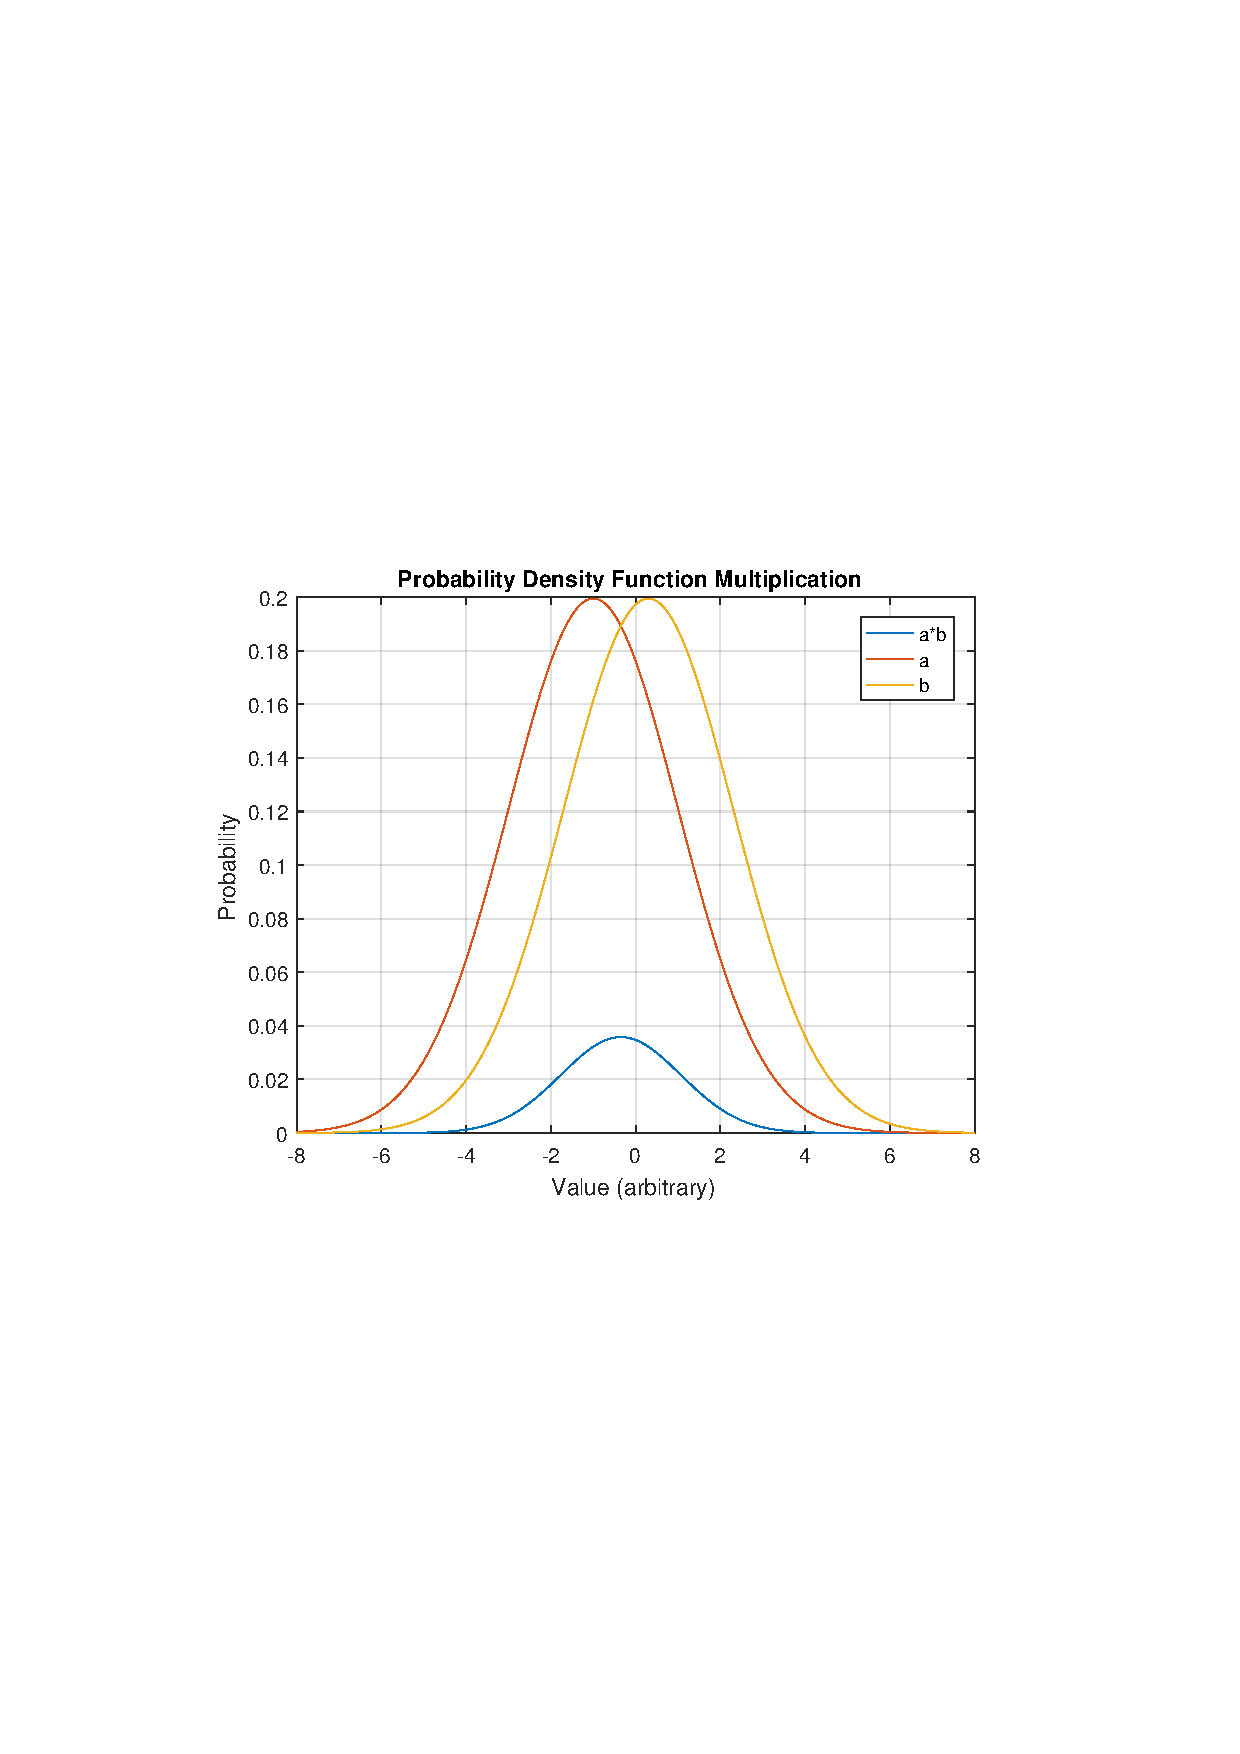
\includegraphics[height=0.35\textheight,trim={0cm 9cm 0cm 9cm},clip]{pdfmultiplication.pdf}
	\mycaption[Probability Distribution Multiplication]{Graph showing the result of multiplying two probability distributions together. The result would then be renormalised to have a total probability of one.}
	\label{fig:gaussiancombination}
\end{figure}

\section{Step by Step Analysis of the Filter}
Starting with the simple case where the one-dimensional vertical position and velocity of the drone needs to be estimated. The state here will be a vector containing the estimation means as shown:
\[\chi 
=
\left |  \begin{array}{c}
pos \\
vel
\end{array}  \right |\]

with an associated covariance matrix:
\[ P 
= 
\left |  \begin{array}{cc}
\sigma_{pp} & \sigma_{pv} \\
\sigma_{vp} & \sigma_{vv}
\end{array}  \right |\]


Assuming there are two sensors, one measuring the height of the drone in meters (m), and one measuring the vertical velocity of the drone in meters per second (m/s). Their values will be stored in the vector:
\[z 
=
\left |  \begin{array}{c}
posMeas \\
velMeas
\end{array}  \right |\]

also with an associated covariance matrix:
\[R 
= 
\left |  \begin{array}{cc}
\sigma_{pMpM} & \sigma_{pMvM} \\
\sigma_{vMpM} & \sigma_{vMvM}
\end{array}  \right |\]

In the case of independent sensors, as is often the case, the covariance matrix will be diagonal.
It is worth noting that the accuracy of the filter relies heavily on the accuracy of the covariance matrices and hence on proper characterisation of the state and the measurement apparatus.\par
From here the filter proceeds sequentially with step \textit{n} being derived from step \textit{n-1} combined with the control inputs and measurement readings.

The Kalman filter only ever uses the last time step to calculate the next, along with any information gained through control inputs or sensors. An initial state is required to begin the algorithm; while an accurate starting point is certainly very helpful, the filter will converge towards the true state fairly quickly.

\subsection{Step One: Extrapolation with Control Input}
\subsubsection{Extrapolation}
From the state values in the previous time step we can extrapolate to where we expect the state values to be now. Intuitively, the previous position and velocity will have an effect on the new position while only the previous velocity will effect the new velocity. Formally written from simple kinematic principals:
\[pos_n = pos_{n-1} + \Delta t vel_{n-1}\]
\[vel_n = vel_{n-1}\]

In matrix form:
\[\left |  \begin{array}{c}
pos_n \\
vel_n
\end{array}  \right |
= 
\left |  \begin{array}{cc}
1 & \Delta t \\
0 & 1
\end{array}  \right |
\left |  \begin{array}{c}
pos_{n-1} \\
vel_{n-1}
\end{array}  \right |\]

This transformational matrix is known as the state transition matrix, denoted \textit{F},  and details how each variable in the state matrix effects every other when we extrapolate to the next time step.\par 
	Having updated the prediction the covariance now also needs updating. Using the identity:
\[Cov(\chi) = \sigma\]
\[Cov(A\chi) = A \sigma A^T\]
It can be shown that since:
\[\hat{\chi}_{n|n-1} = F\chi_{n-1|n-1} \]
then:
\[P_{n|n-1} = FP_{n-1|n-1}F^T\]

\subsubsection{Control input}
	At this stage any control levers can be introduced to the model. In this example, we will look at the idea of the drone having control over its acceleration. The acceleration can be introduced into the system using a similar style of matrix to that used in the extrapolation earlier where each element represents the effect of a control lever on every part of the state. This matrix is referred to as the input or control matrix, denoted \(B\), and will be described in this example as:
\[B
=
\left |  \begin{array}{c}
dt^2/2 \\
dt
\end{array}  \right |\]

from the kinematic equations:
\[pos_n = pos_{n-1} + \Delta t\, vel_{n-1} + \frac{1}{2} u\, \Delta t^2\]
\[vel_n = vel_{n-1} + u\, \Delta t\]
where u = acceleration.

The control process has its own associated variance caused by imperfect application in a real world environment; in this example for instance variance could be introduced through turbulence. Here the variance \(Q\) will simply be:
\[Q 
=
\textrm{input variance}
\times
BB^T\]

\subsubsection{Overall}
The combined overall equations for this step are:
\[\hat{\chi}_{n|n-1} = F\hat{\chi}_{n-1|n-1} + Bu\]
where \textit{u} is the input acceleration, and:
\[P_{n|n-1} = FP_{n-1|n-1}F^T + Q\]
describes the covariance update.

\subsection{Step Two: Measurements Update}
Now that there is a first estimate for where the drone should be based on the information available from the last step, the measurement information acquired this step can be utilised. Once again there will be a mean estimate value for each sensor (i.e. the reading) and an associated covariance matrix for the sensory apparatus as a whole. \par
\subsection{Mapping the Readings to the State}
	Firstly there needs to exist an association matrix which maps the measurements vector onto the state space. In this example where we have the measurement vector:
\[z 
=
\left |  \begin{array}{c}
posMeas \\
velMeas
\end{array}  \right |\]

the association matrix is simply:
\[H 
=
\left |  \begin{array}{cc}
1 & 0 \\
0 & 1
\end{array}  \right |\]

showing that the measured position has a one-to-one relationship with the state position, no relationship to the state velocity and vice versa for the measured velocity.\par

\subsubsection{The Innovation Vector}
	From the measurement vector containing the sensor readings the innovation vector is derived. This describes the measurement residual or, more intuitively, the difference between each reading and the state estimate from step one and is given by:
  \[Inn 
  =
  z - H\hat{\chi}_{n|n-1}\]
  The covariance of this innovation vector is derived from the estimation covariance and the measurement covariance as shown:
\[\sigma_{Inn}
=
H P_{n|n-1} H^T + R\]

\subsubsection{Combination Through the Kalman Gain}
The innovation now needs to be combined with the step one estimate to give an overall prediction of the state. The Kalman gain is used to weight the two previous steps, and can be thought of as the proportional confidence of the measurements relative to our extrapolated state prediction from step one. It should therefore be intuitive that the Kalman gain is derived from the covariances which describe the probable error. The Kalman gain is given in the equation below:
\[K
=
\frac{P_{n|n-1} H^T}{\sigma_{Inn}}\]

The state estimate can now be updated simply with the equation:
\[\hat{\chi}_{n|n}
=
\hat{\chi}_{n|n-1} + K\, Inn\]

The final step then is to calculate the new covariance of the state estimate \(P_{n|n}\) as to be used in the next algorithm iteration using:
\[P_{n|n}
=
P_{n|n-1} - K H P_{n|n-1}\]

\subsection{Summary}
The transition (\(F\)), control/input (\(B\)) and measurement (\(H\)) matrices stay the same throughout the entire filter run time as they are defined by equations for physical laws and are not dependent on any of the run time variables. The covariance matrix describing sensor noise is also constant, however it may be a function of other factors such as the current measurement e.g. the noise may increase as a measured distance increases.













